\documentclass[tikz,border=8pt]{standalone}
\usetikzlibrary{arrows.meta}
\begin{document}
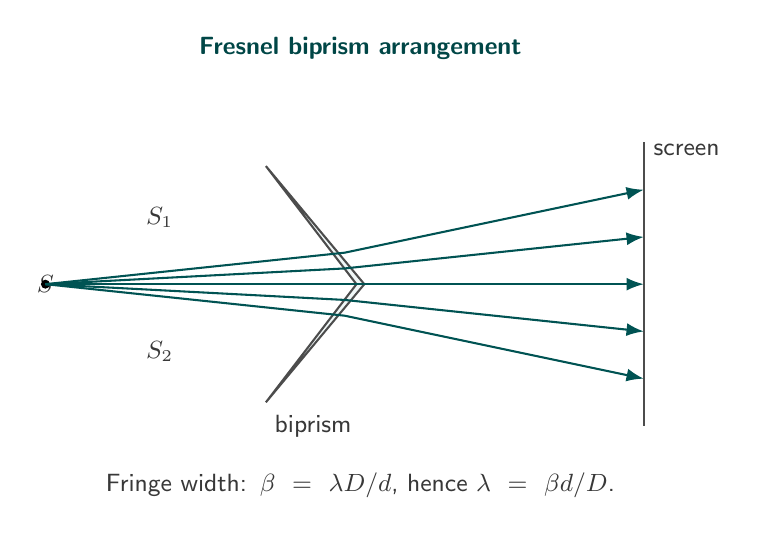
\begin{tikzpicture}[
  ray/.style={-{Latex[length=2.2mm]},draw=teal!65!black,line width=0.75pt},
  line/.style={draw=black!70,line width=0.75pt},
  label/.style={font=\sffamily\small,text=black!78},
  title/.style={font=\sffamily\bfseries\small,text=teal!55!black},
]
\node[title] at (0,3.0) {Fresnel biprism arrangement};
\node[label] at (-4,0) {$S$};
\draw[fill=black] (-4,0) circle (1.4pt);
\draw[line,fill=teal!6] (-1.2,1.5)--(-0.05,0)--(-1.2,-1.5)--(0.05,0)--cycle;
\node[label] at (-0.6,-1.8) {biprism};
\draw[line] (3.6,-1.8)--(3.6,1.8);
\node[label,right] at (3.6,1.7) {screen};
\foreach \y in {-1.2,-0.6,0,0.6,1.2}{\draw[ray] (-4,0)--(-0.2,\y/3)--(3.6,\y);}
\node[label] at (-2.55,0.85) {$S_1$};
\node[label] at (-2.55,-0.85) {$S_2$};
\node[label,align=center,text width=8.2cm] at (0,-2.55)
  {Fringe width: $\beta=\lambda D/d$, hence $\lambda=\beta d/D$.};
\end{tikzpicture}
\end{document}
